\section{PWM-Grundlagen und Modulation}
\subsection*{Definition der verwendeten Grössen}

\begin{itemize}
    \item $u_{\mathrm{ref}}(t)$: Referenzspannung (Sinus),
    \item $u_{\mathrm{tri}}(t)$: Trägerspannung (Dreieck),
    \item $\hat U_{\mathrm{ref}}$: Scheitelwert der Referenzspannung,
    \item $\hat U_{\mathrm{tri}}$: Scheitelwert der Trägerspannung,
    \item $m_a$: Amplitudenmodulationsindex,
    \item $f_1$: Grundfrequenz der Referenz,
    \item $f_s$: Träger- bzw. Schaltfrequenz,
    \item $U_{DC}$: Zwischenkreisspannung.
\end{itemize}

\subsection{Grundidee der Pulsweitenmodulation}

% --- bestehende Grafik: Sinus-Dreieck-Vergleich ---
\begin{center}
    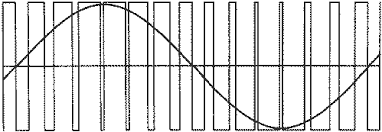
\includegraphics[width=0.85\linewidth]{images/sinuspwm.png}
\end{center}

Bei der Sinus-PWM wird:

\begin{itemize}
    \item Referenz: $u_{\mathrm{ref}}(t) = \hat U \sin(\omega t)$
    \item Träger: Dreieckspannung mit Frequenz $f_s$
\end{itemize}

Schaltregel:
\[
\text{Schalter EIN, wenn } u_{\mathrm{ref}}(t) > u_{\mathrm{tri}}(t)
\]

\subsection{Modulationsgrad}

\[
\cbl{m = \frac{\hat U_{\mathrm{ref}}}{\hat U_{\mathrm{tri}}}}
\]

Grundschwingungsamplitude:
\[
\cbl{\hat U_1 = m \cdot U_{DC}}
\]

Aussage:
\begin{itemize}
    \item $0 \le m \le 1$ linearer Modulationsbereich
    \item Amplitude proportional zu $m$
\end{itemize}

\subsection{Schaltfrequenz}

\[
\cbl{f_s \gg f_1}
\]

Eigenschaften:
\begin{itemize}
    \item Hohe $f_s$ $\Rightarrow$ gute Spektralqualität
    \item Hohe $f_s$ $\Rightarrow$ höhere Schaltverluste
\end{itemize}
\subsection{Grundschwingungsamplitude bei Sinus-PWM}

Für lineare Modulation ($m_a \le 1$) gilt:

\[
\boxed{\hat U_1 = m_a \frac{U_{DC}}{2}}
\]

Effektivwert:
\[
\boxed{U_{1,\mathrm{RMS}} = m_a \frac{U_{DC}}{2\sqrt{2}}}
\]

\subsection{Spektrum der PWM}

% --- bestehende Grafik: PWM-Spektrum ---
\begin{center}
    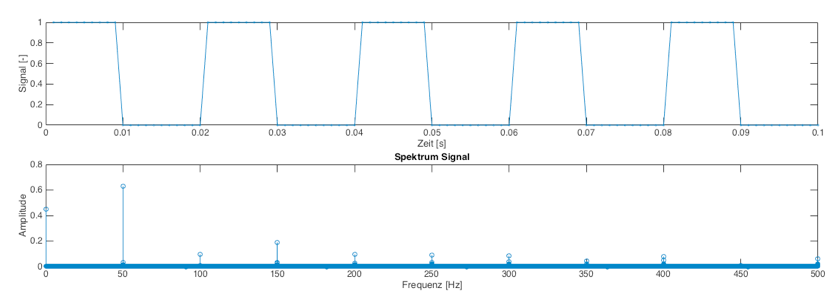
\includegraphics[width=0.85\linewidth]{images/specpwm.png}
\end{center}
Eigenschaften:
\begin{itemize}
    \item Grundschwingung bei $f_1$
    \item Seitenbänder um Vielfache von $f_s$
    \item Tiefpassfilter erzeugt nahezu Sinus
\end{itemize}

\crd{\textrightarrow\ PWM erlaubt getrennte Einstellung von Frequenz und Amplitude.}
